\item Obtener toda la información de los clientes que viven en New York o en Washington, que pertenezcan al segmento consumer que hayan solicitado una orden en el tercer trimestre de 2016. Mostrar la información ordenada por la cantidad solicitada.

\begin{lstlisting}
residencia = σ state = 'New York' ∨ state = 'Washington' (customer)

segmento = σ segment = 'Consumer' (residencia)

trimestre = σ orderdate ≥ date('2016-07-01') ∧ orderdate ≤ date('2016-09-30') (orders)

resultado = π customerid,customername,segment,country,city,state,postalcode,region,quantity (segmento ⨝ trimestre)

τ quantity ASC (resultado)
\end{lstlisting}

\begin{center}
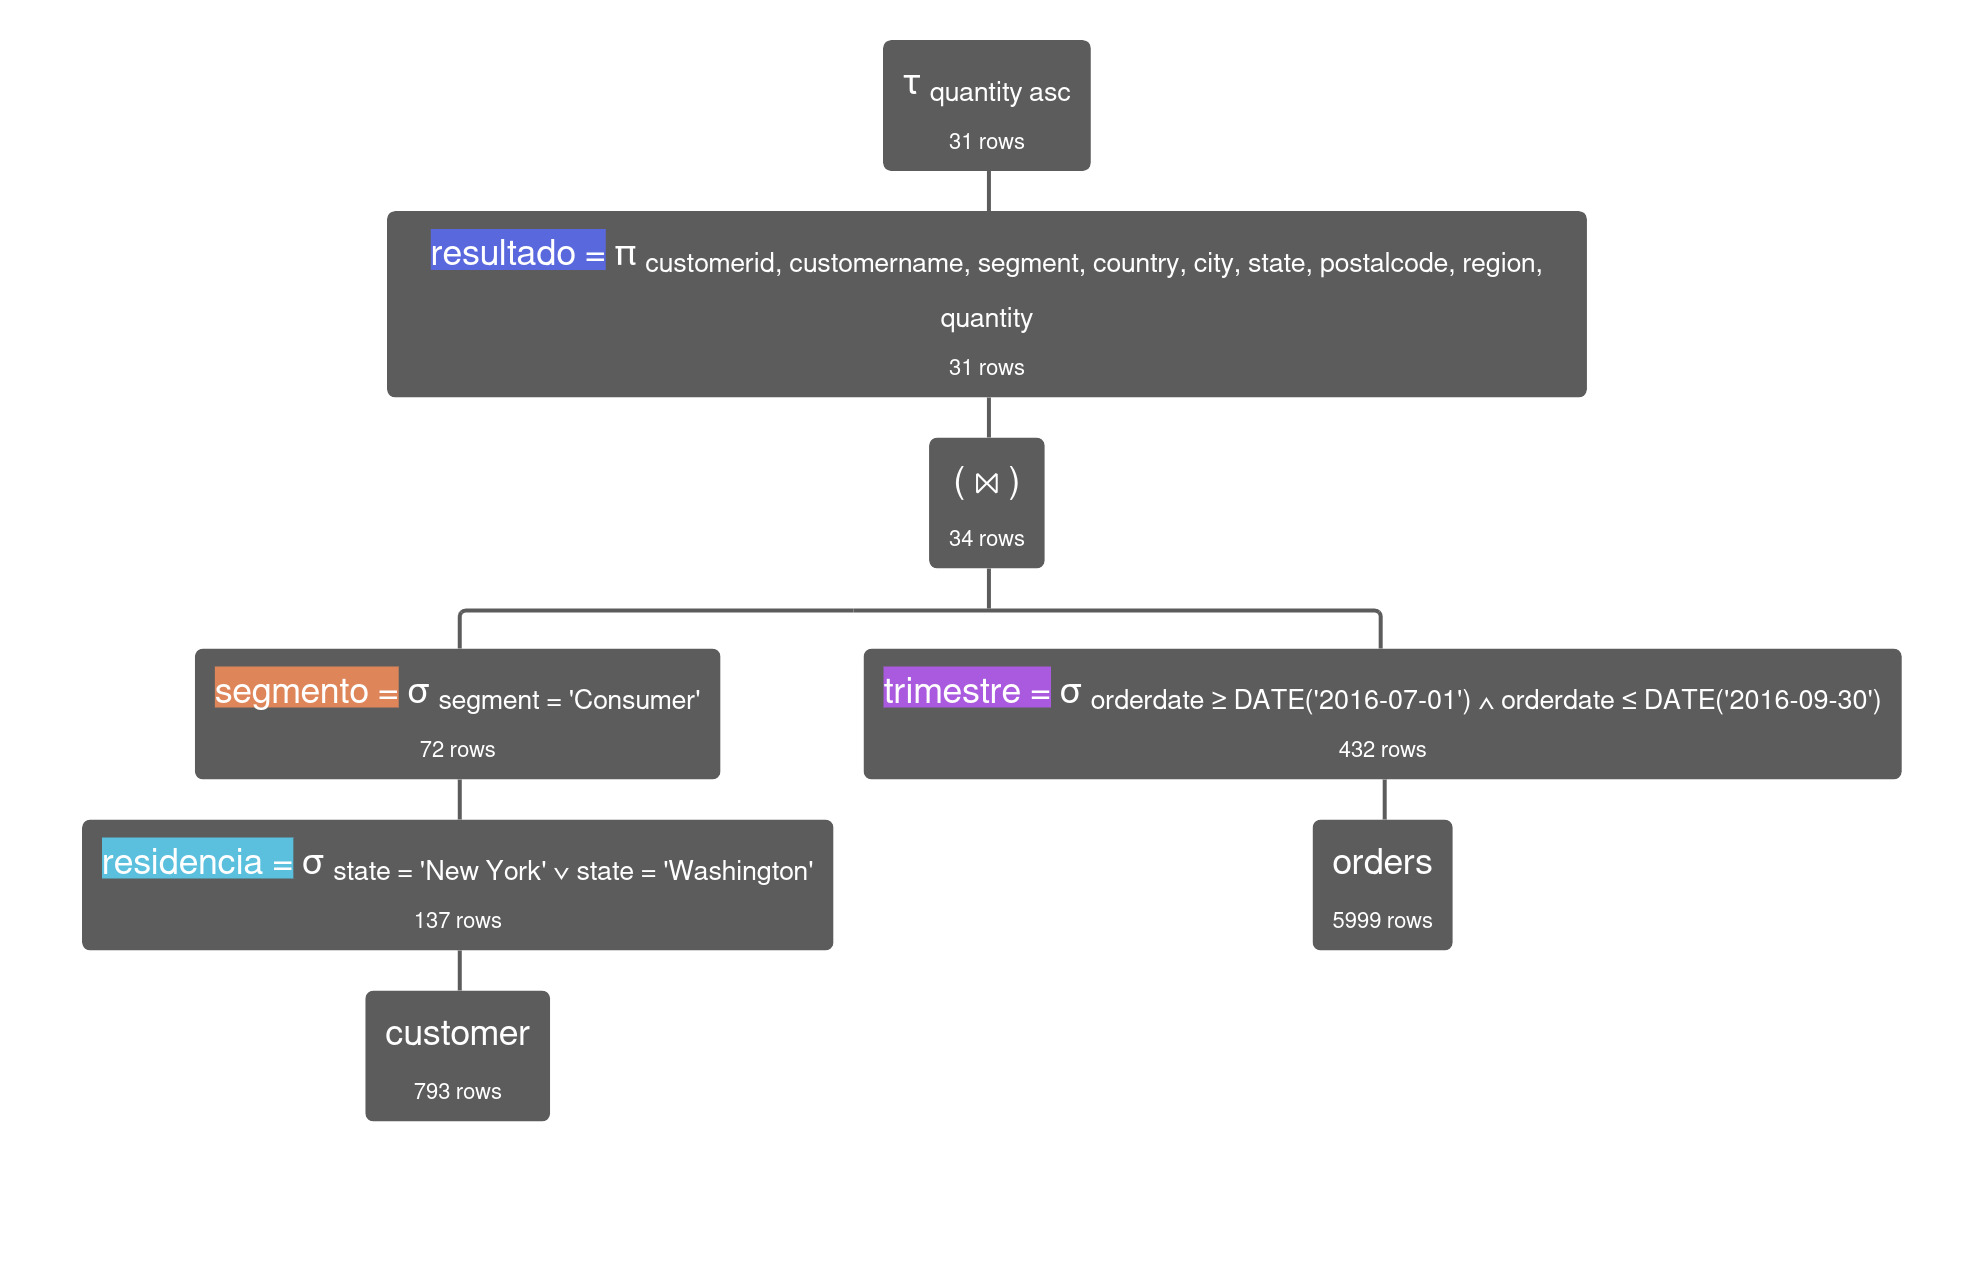
\includegraphics[width=0.7\textwidth]{figuras/2a_arbol.jpg}
\end{center}

\begin{center}
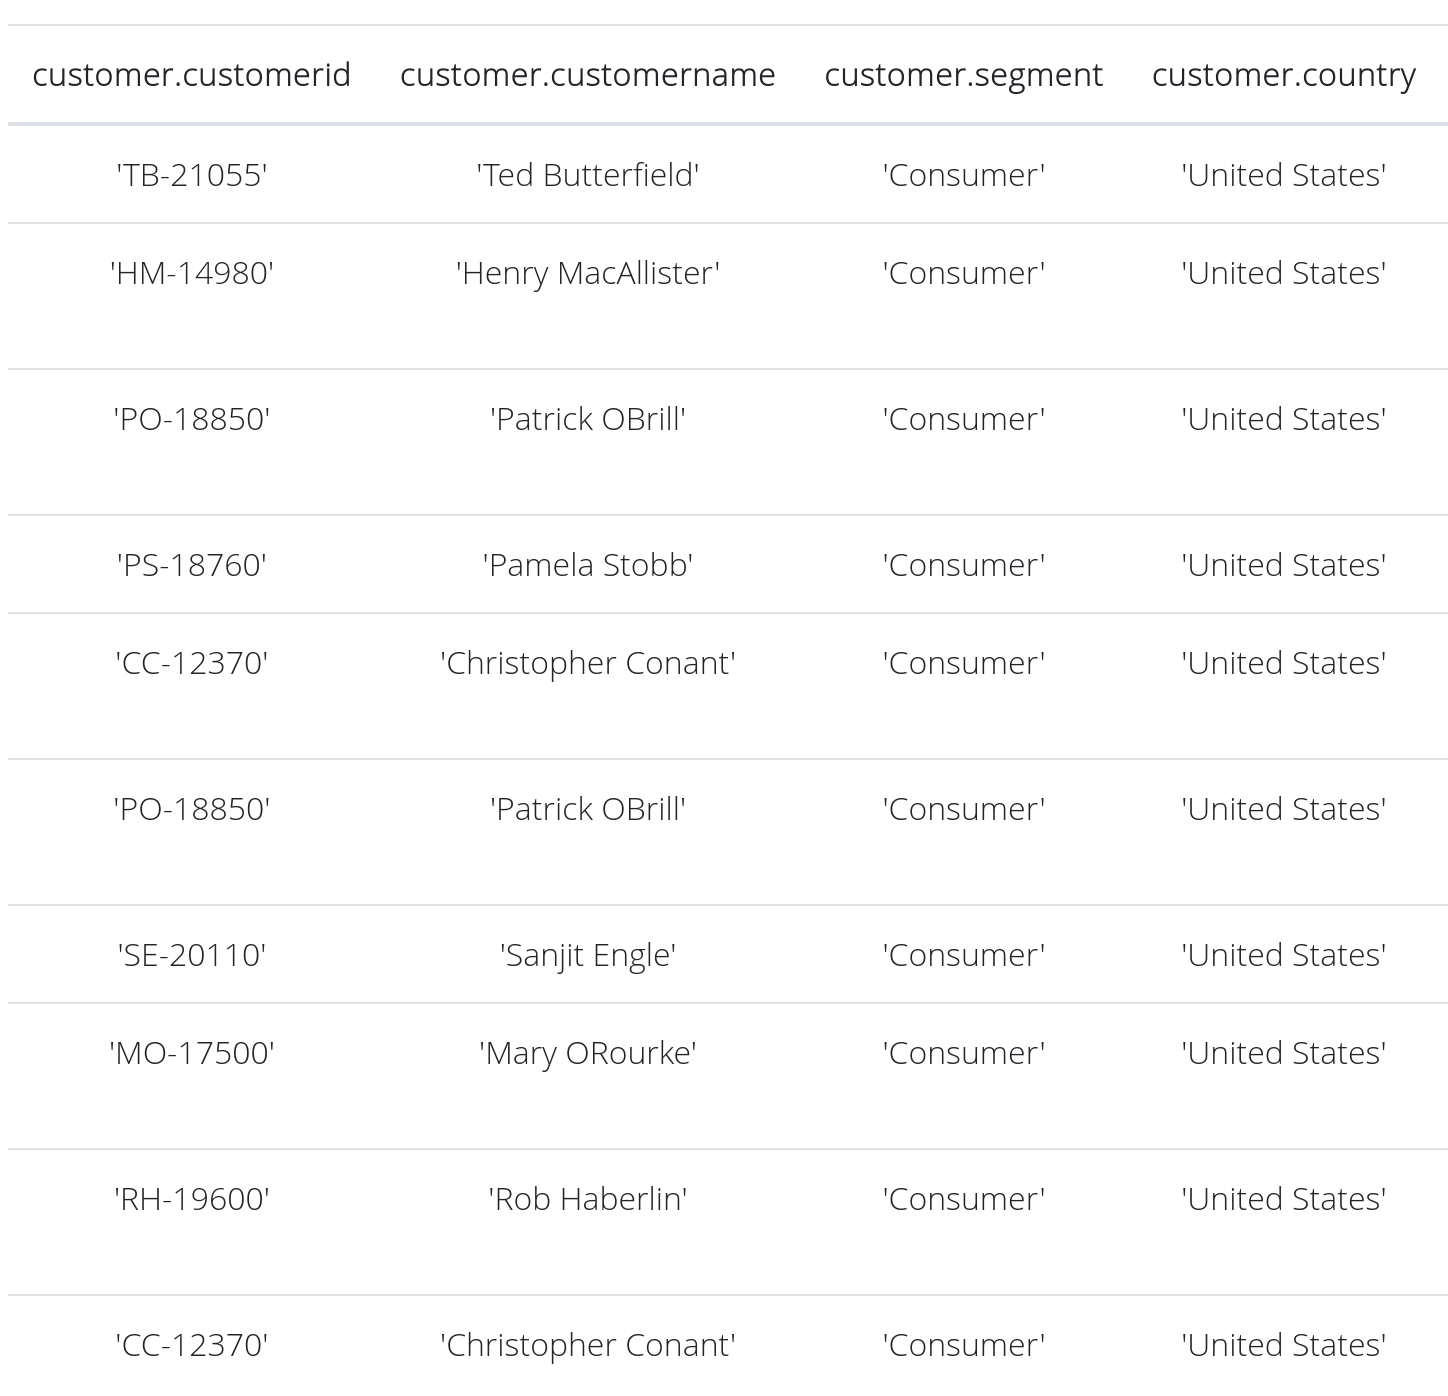
\includegraphics[width=0.38\textwidth]{figuras/2a_tuples.png}
\end{center}

\newpage
